\documentclass[14pt]{beamer}
\usepackage[T2A]{fontenc}
\usepackage[utf8]{inputenc}
\usepackage[english]{babel}
\usepackage{amssymb,amsfonts,amsmath,mathtext}
\usepackage{cite,enumerate,float,indentfirst}
\usepackage{graphicx}
\usepackage{multicol}
\usepackage[boxed,algochapter,noline,czech]{algorithm2e}

\renewcommand{\vec}[1]{\ensuremath{\boldsymbol{#1}}}

\graphicspath{{images/}}

\usetheme{Pittsburgh}
\usecolortheme{whale}

\setbeamercolor{footline}{fg=blue}
\setbeamertemplate{footline}{
  \leavevmode%
  \hbox{%
  \begin{beamercolorbox}[wd=.333333\paperwidth,ht=2.25ex,dp=1ex,center]{}%
    Boris Kudryashov, ITMO University
  \end{beamercolorbox}%
  \begin{beamercolorbox}[wd=.333333\paperwidth,ht=2.25ex,dp=1ex,center]{}%
    St. Petersburg, 2016
  \end{beamercolorbox}%
  \begin{beamercolorbox}[wd=.333333\paperwidth,ht=2.25ex,dp=1ex,right]{}%
  Page \insertframenumber{} of \inserttotalframenumber \hspace*{2ex}
  \end{beamercolorbox}}%
  \vskip0pt%
}

\newcommand{\itemi}{\item[\checkmark]}

\title{\small{Information Theory. 2nd Chapter Slides}}
\author{\huge{
Boris Kudryashov \\
\vspace{30pt}
ITMO University
}}


\begin{document}

\maketitle

\begin{frame}
\frametitle{Agenda}
\begin{enumerate}    
% \footnotesize {
% \small{
    
    \item Uneven letter-by-letter coding
    \item Kraft inequality
    \item Letter-by-letter coding theorems
    \item Huffman code
    \item Huffman code redundancy
    \item Shannon code
    \item Gilbert-Moore code
    \item Stationary source coding

\end{enumerate}
\end{frame}

% ------------------letter-by-letter coding---------------

\begin{frame}
\frametitle{Letter-by-letter coding}
Example: $X = \{0,1,2,3\}$
\begin{itemize}    
% \footnotesize {
% \small{

    \item $C_1 = \{00,01,10,11\}$;
    \item $C_2 = \{1,01,001,000\}$;
    \item $C_3 = \{1,10,100,000\}$ ;
    \item $C_4 = \{0,1,10,01\}$;
    
    \item
    \begin{figure}[ht]
    \begin{minipage}{1.0\linewidth}
    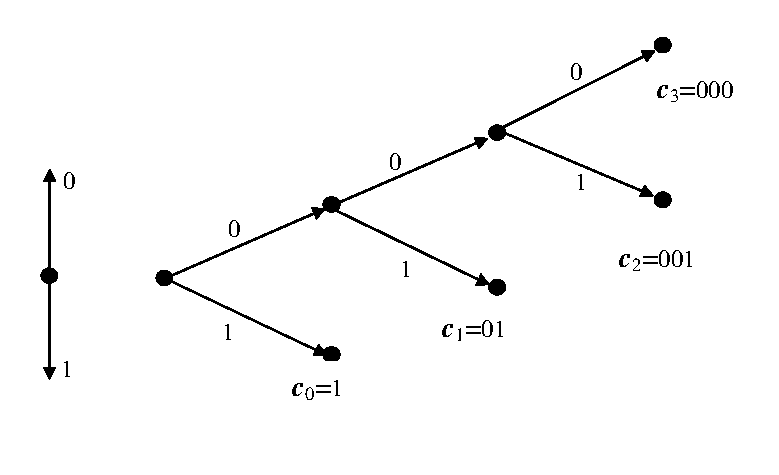
\includegraphics[width=0.9\textwidth]{fig2_1.eps}
    \caption{Binary code tree example} \label{code_ex}
    \end{minipage}
    \end{figure}

\end{itemize}
\end{frame}


\begin{frame}
\frametitle{Letter-by-letter coding}
\begin{itemize}    
% \footnotesize {
% \small{

    \item Consider $X = \{1,...,M\}$, $\{p_1 ,...,p_M \}$.
    $C = \{\vec c_1 ,...,\vec c_M \}$, codewords $l_1,\dots,l_M$.
    
    \item  Average codeword length
    \[
    \bar {l} = {\rm {\bf M}}[l_i ] = \sum\limits_{i = 1}^M {p_i l_i } 
    \]

\end{itemize}
\end{frame}

% ---------------------Kraft inequality-------------

\begin{frame}
\frametitle{Kraft inequality}
% \footnotesize {
% \small{

    \begin{theorem} {Kraft inequality}
    \label{Kraft_ineq}
    Prefix code of size $M$ with codewords of length $l_1 ,...,l_M $ exists iff Kraft inequality holds:
    \begin{equation}
    \label{Kraft} \sum\limits_{i = 1}^M {2^{ - l_i } \le 1} .
    \end{equation}
    \end{theorem}
\end{frame}


\begin{frame}
\frametitle{Kraft inequality}
Proof of theorem
\begin{itemize}    
% \footnotesize {
\small{

    \item Consider $L$, such that $L \ge \max _i l_i $. 
    \[
    \sum\limits_{i = 1}^M {2^{L - l_i } \le 2^L} .
    \]
    
    \item Consider:
    \begin{figure}[ht]
    \begin{minipage}{1.0\linewidth}
    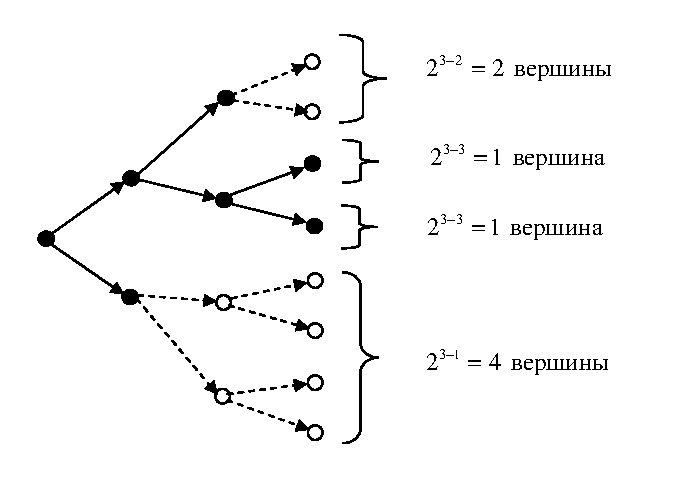
\includegraphics[width=0.7\textwidth]{fig2_2.eps}
    \caption{Clarification to Kraft inequality proof for Prefix code existence.} \label{Kraft_nec}
    \end{minipage}
    \end{figure}
    
}
\end{itemize}
\end{frame}


\begin{frame}
\frametitle{Kraft inequality}
Proof of theorem
\begin{itemize}    
% \footnotesize {
% \small{

    \item 
    \[
    2^{l_2 } - 2^{l_2 - l_1 } \ge 1
    \]
    
    \item
    \[
    2^{l_3 } - 2^{l_3 - l_2 } - 2^{l_3 - l_1 } \ge 1
    \]
    
    \item
    \[
    2^{l_M } - 2^{l_M - l_{M - 1} } - 2^{l_M - l_{M - 2} } - ... - 2^{l_M - l_1}
    \]


\end{itemize}
\end{frame}



\begin{frame}
\frametitle{Kraft inequality}
\begin{itemize}
% \footnotesize {
% \small{

    \item $l_1 = 1$, $l_2 = 2$, $l_3 = l_4 = 3$. 
    \begin{figure}[ht]
    \begin{minipage}{1.0\linewidth}
    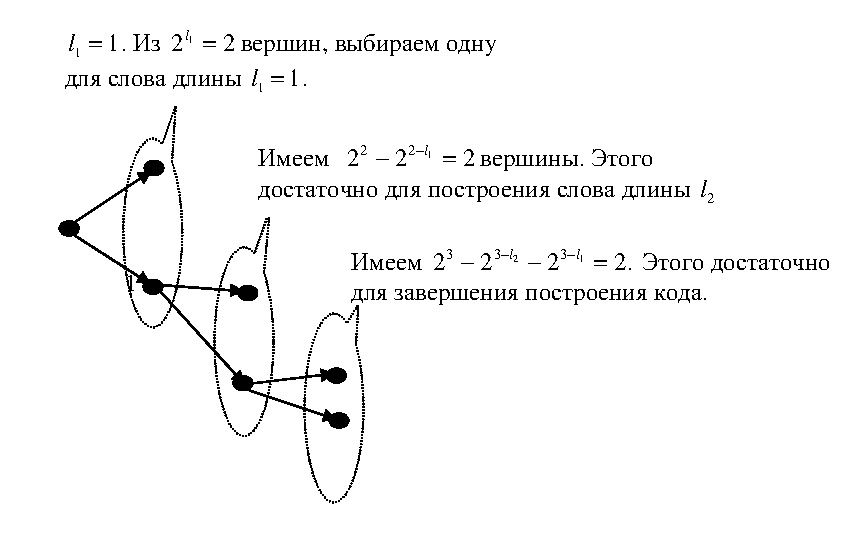
\includegraphics[width=1.0\textwidth]{fig2_3.eps}
    \caption{Binary code tree construction.} \label{Kraft_en}
    \end{minipage}
    \end{figure}

\end{itemize}
\end{frame}



\begin{frame}
\frametitle{Kraft inequality}
% \footnotesize {
% \small{

    \begin{theorem} For any uniquely decoded binary code of size $M$ with codeword length $l_1 ,...,l_M $ holds
    \begin{equation}
    \label{Kraft2} \sum\limits_{i = 1}^M {2^{ - l_i } \le 1} .
    \end{equation}
    \end{theorem}
    
\end{frame}


\begin{frame}
\frametitle{Kraft inequality}
Proof of Theorem
\begin{itemize}    
% \footnotesize {
\small{

    \item Consider $N \in \mathbb{N}$
    \begin{eqnarray*}
     \left( {\sum\limits_{i = 1}^M {2^{ - l_i }} }
    \right)^N &=& \underbrace {\left( {\sum\limits_{i_1 = 1}^M {2^{ -
    l_{i_1 } }} } \right)...\left( {\sum\limits_{i_N = 1}^M {2^{ -
    l_{i_N } }} } \right)}_{N\mbox{ factors}} = \\
    &=&\sum\limits_{i_1 = 1}^M {...\sum\limits_{i_N = 1}^M {2^{ -
    (l_{i_1 } + ... + l_{i_N } )}} } .
    \end{eqnarray*}

    \item 
    \[
    \left( {\sum\limits_{i = 1}^M {2^{ - l_i }} } \right)^N = \sum\limits_{L =
    1}^{Nl_M } {A_L 2^{ - L}} .
    \]
}
\end{itemize}
\end{frame}


\begin{frame}
\frametitle{Kraft inequality}
\begin{itemize}    
% \footnotesize {
% \small{

    \item
    \[
    \left( {\sum\limits_{i = 1}^M {2^{ - l_i }} } \right)^N \le \sum\limits_{L =
    1}^{Nl_M } {2^L2^{ - L} = Nl_M } .
    \]
    
    \item $N$-th root:
    \[
    \sum\limits_{i = 1}^M {2^{ - l_i }} \le \left( {Nl_M } \right)^{1 / N} = 2^{\frac{\log (Nl_M )}{M}}.
    \]
        
\end{itemize}
\end{frame}



\begin{frame}
\frametitle{Coding Theorems}  
% \footnotesize {
% \small{

    \begin{theorem}{Achievability Theorem.}
    \label{PTK}
    For ensemble $X = \{x,p(x)\}$ with entropy $H$ there exists letter-by-letter uneven prefix code with average codeword length $\bar {l} < H + 1$. \end{theorem}

\end{frame}


\begin{frame}
\frametitle{Coding theorems}
Achievability Theorem Proof
\begin{itemize}    
% \footnotesize {
% \small{
    
    \item Consider  $X = \{1,...,M\}$, $p_1 ,...,p_M $. 
    \item $x_m <-> l_m = \left\lceil { - \log p_m } \right\rceil $, $m = 1,...,M.$ 
   
    \item Codeword length satisfies Kraft inequality:
    \[
    \sum\limits_{m = 1}^M {2^{ - l_m }} = \sum\limits_{m = 1}^M {2^{ - \left\lceil { - \log p_m } \right\rceil }} \le \\
    \le \sum\limits_{m = 1}^M {2^{\log p_m }} = \sum\limits_{m = 1}^M {p_m = 1} .
    \]

\end{itemize}
\end{frame}


\begin{frame}
\frametitle{Coding theorems}
Achievability Theorem Proof
\begin{itemize}    
% \footnotesize {
\small{

    \item Average codeword length:
    \begin{eqnarray*}
    \bar {l} &=& \sum\limits_{m = 1}^M {p_m l_m }=\\
    &=& \sum_{m = 1}^M p_m \left\lceil  - \log p_m  \right \rceil < \\
    &<& \sum_{m = 1}^M p_m \left(  - \log p_m + 1 \right) = \\
    &=& H + \sum\limits_{m = 1}^M p_m =\\
    &=& H + 1 ,
    \end{eqnarray*}
}
\end{itemize}
\end{frame}


\begin{frame}
\frametitle{Coding theorems}  
% \footnotesize {
% \small{

\begin{theorem}{Inverse Theorem.} For any uniquely decoded code of discrete source $X = \{x,p(x)\}$ with entropy $H$, average codeword length $\bar {l}$ satisfies:
\begin{equation}
\label{Inv_Th} \bar {l} \ge H.
\end{equation}
\end{theorem}
    
\end{frame}


\begin{frame}
\frametitle{Coding theorems}
Proof Inverse Theorem
\begin{itemize}    
\footnotesize {
% \small{

    \item Let $l(x)$ be the codeword length for message $x$. 
    \[
    H - \bar {l} = - \sum\limits_{x \in X} {p(x)\log p(x)} - \sum\limits_{x \in
    X} {p(x)l(x) = \sum\limits_{x \in X} {p(x)\log \frac{2^{ - l(x)}}{p(x)}} }
    .
    \]
    \item Use Kraft inequality:
    \[
    \log x \le (x - 1)\log e,
    \]

    \item We get
    \begin{eqnarray}
    \label{part2eq4} H - \bar {l} &\le& \log e\sum\limits_{x \in X} 
    {p(x)\left( {\frac{2^{ - l(x)}}{p(x)} - 1} \right)} =\nonumber\\
    &=& \log e\left( {\sum\limits_{x \in X} {2^{ - l(x)}} - \sum\limits_{x \in X} {p(x)} } \right)\le \nonumber\\ 
    & \le& \log e\left( {1 - \sum\limits_{x \in X} {p(x)} } \right) = 0.
    \end{eqnarray}
}
\end{itemize}
\end{frame}


\begin{frame}
\frametitle{Huffman code}
Properties of Huffman code
\begin{itemize}    
% \footnotesize {
% \small{

    \item[1]
    \begin{prop} If $p_i < p_j $, the $l_i \ge l_j $.
    \label{HProp1}
    \end{prop}
    
    \item[2]
    \begin{prop}
    \label{HProp2} At least two codewords have the same langth
    $l_M = \max _m l_m $.
    \end{prop}
    
    \item[3]
    \begin{prop}
    \label{HProp3} There are two codewords of length $l_M = \max _m l_m $ which differ only in the last character.
    \end{prop}
    
    \item[4]
    \begin{prop}
    \label{HProp4} If code $C'$ for $X'$ is optimal, then, code $C$
    is optimal for  $X$.
    \end{prop}

\end{itemize}
\end{frame}


\begin{frame}
\frametitle{Huffman code}
\footnotesize {
Proof of property 4
% \small{
   
    \[
    l_m = \left\{ {{\begin{array}{*{20}c}
     {{l}'_m \mbox{ при }m \le M - 2,} \hfill \\
     {{l}'_{M - 1} + 1\mbox{ при }m = M - 1,M.} \hfill \\
    \end{array} }} \right.
    \]

    \begin{eqnarray*}
    \bar {l} &=& \sum\limits_{m = 1}^M {p_m l_m } =\\
    &=& \sum\limits_{m = 1}^{M - 2} {p_m l_m + p_{M - 1} l_{M - 1} +
    p_M l_M} = \\
    &=& \sum\limits_{m = 1}^{M - 2} {p_m l_m + (p_{M - 1} + p_M
    )({l}'_{M - 1} + 1) }=\\
    &=& \sum\limits_{m = 1}^{M - 2} {{p}'_m {l}'_m + {p}'_{M - 1} }
    {l}'_{M - 1} + p_{M - 1} + p_M =\\
    &=& \sum\limits_{m = 1}^{M - 1} {{p}'_m {l}'_m + p_{M - 1} + p_M =
    {\bar {l}}'} + p_{M - 1} + p_M .
    \end{eqnarray*}
    where $\bar {l}'=\sum\limits_{m = 1}^{M - 1} p'_m l'_m$ is average codeword length of code $C'$. 
}
\end{frame}

\begin{frame}
\frametitle{Huffman code}
\begin{itemize}    
% \footnotesize {
% \small{


    \begin{center}
    \begin{figure}
    \scalebox{0.75}{
    \begin{algorithm}[H]
      \dontprintsemicolon
      \KwIn{Alphabet size $M$, probabilities of characters }
      \KwOut{Bitary tree of Huffman code}
      \BlankLine
      \CommentSty{Init:}
      number of unprocessed nodes $M_0=M$ 
      \While{$M_0>1$}
      {
            Find two unprocessed nodes with min probabilities.
            Exclude these nodes from the list of unprocessed.
            Introduce new node, attribute to him the total probability of two excluded nodes.
            Bind new node with edges to two excluded node.
            $M_0 \leftarrow M_0  - 1$.
       }
    \end{algorithm}
    }
    \caption{Building Huffman code tree }
    \label{alg_huf}
    \end{figure}
    \end{center}


\end{itemize}
\end{frame}


\begin{frame}
\frametitle{Huffman code}
\begin{itemize}    
% \footnotesize {
% \small{

\begin{figure}[ht]
\begin{minipage}{1.0\linewidth}
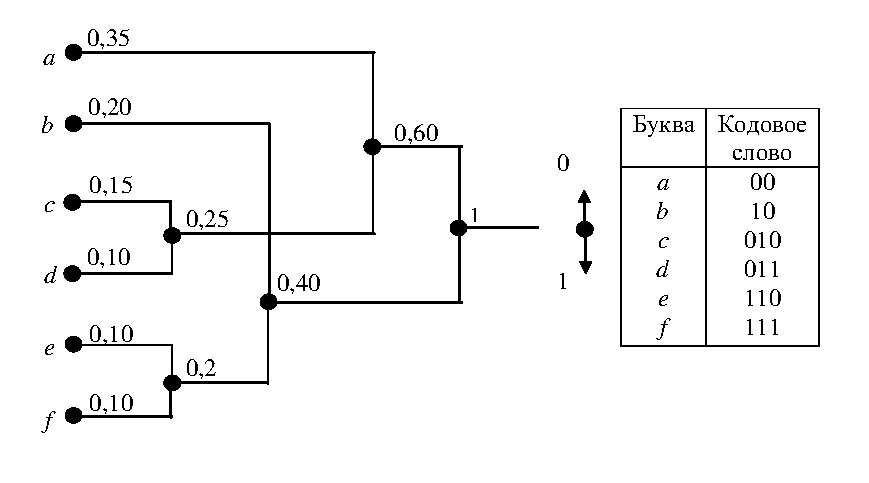
\includegraphics[width=0.9\textwidth]{fig2_4.eps}
\caption{Huffman code example} \label{Huf_ex}
\end{minipage}
\end{figure}

\end{itemize}
\end{frame}

% -----------------------Huffman code redundancy--------------

\begin{frame}
\frametitle{Huffman code redundancy}  
% \footnotesize {
% \small{

\begin{theorem} \label{th_huf_red}
Let $p_1 $ be maximal probability of message. Then redundancy of Huffman code for this ensemble satisfies:
    \begin{equation}
    \label{part2eq6} r \le \left\{ {{\begin{array}{*{20}c}
     {p_1 + \sigma ,\mbox{ for }p_1 < 1 / 2,} \hfill \\
     {2 - \eta(p_1 ) - p_1 \mbox{ for }p_1 \ge 1 / 2,} \hfill \\
    \end{array} }} \right.
    \end{equation}
    where $\eta(x) = - x\log x - (1 - x)\log (1 - x)$ is binary ensemble entropy, and
    \begin{equation}
    \label{part2eq7} \sigma = 1 - \log e - \log \log e \approx 0,08607.
    \end{equation}
    \end{theorem}
\end{frame}


\begin{frame}
\frametitle{Huffman code redundancy}
\begin{itemize}    
% \footnotesize {
% \small{

    \begin{center}
    \begin{figure}[htbp]
    \centerline{
    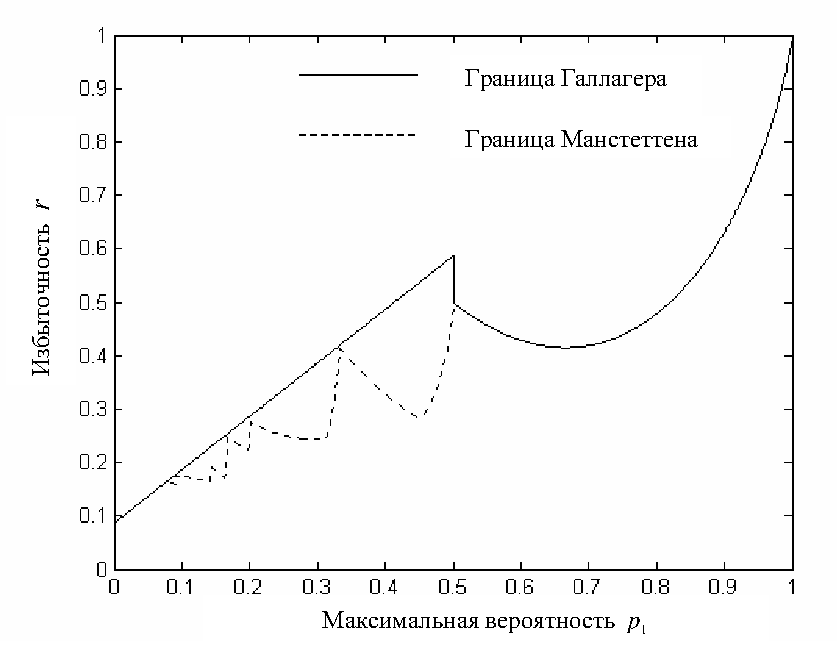
\includegraphics[width=0.8\textwidth]{fig2_5.eps}
    }
    \caption{Huffman code redundancy} \label{HUF_RED}
    \end{figure}
    \end{center}

\end{itemize}
\end{frame}

% --------------------------Shannon code-------------------

\begin{frame}
\frametitle{Shannon code}
\begin{itemize}    
% \footnotesize {
% \small{
    
    \begin{center}
    \begin{figure}
    \scalebox{0.70} {
    \begin{algorithm}[H]
    \dontprintsemicolon
      \KwIn{Alphabet size $M$, character probabilities $p_i, i=1,...,M$ }
      \KwOut{List of Shannon codewords}
      \BlankLine
      \CommentSty{Sorting:}
      \For {$i=1$ \emph{\KwTo} $M$}
      {
      $j(i)\leftarrow$ index of $i$-th descending character probability
      }
      \BlankLine
      \CommentSty{Cumulative probabilities:} 
      $q_{j(1)}=0$;
      \For {$i=2$ \emph{\KwTo} $M$}
      {
      $q_{j(i)}=q_{j(i-1)}+p_{j(i-1)}$;
      }
      \BlankLine
      \CommentSty{Codewords:}
      \For {$i=1$ \emph{\KwTo} $M$}
      {
      $\vec c_i\leftarrow $ first
      $\left\lceil { - \log p_i } \right\rceil $ bits after comma in a binary number $q_i$.
      }
    \end{algorithm}
    }
    \caption{Shannon code construction algorithm}
    \label{alg_sh}
    
    \end{figure}
    \end{center}

\end{itemize}
\end{frame}

\begin{frame}
\frametitle{Shannon code}
\begin{itemize}    
% \footnotesize {
% \small{

\begin{figure}[ht]
%\begin{minipage}{1.0\linewidth}
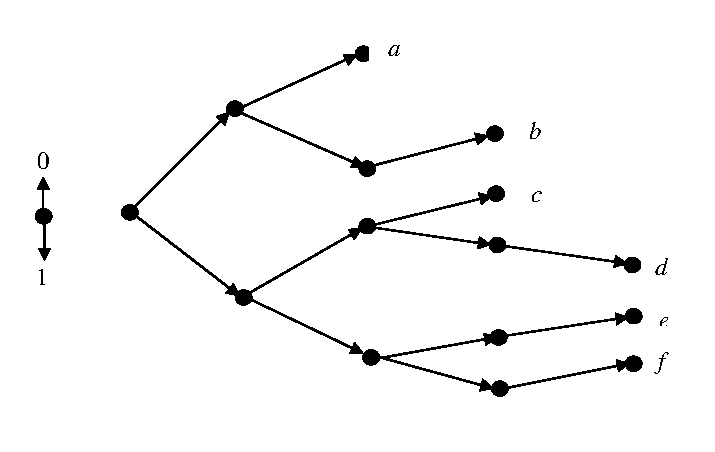
\includegraphics[width=0.85\textwidth]{fig2_6.eps}
%\includegraphics[width=1.0\textwidth]{ttt.eps}
\caption{Shannon codetree for $X =
\{a,b,c,d,e,f\}$, $\{0,35, 0,2, 0,15,
0,1, 0,1, 0,1\}$} \label{Shan_tree}
%\end{minipage}
\end{figure}

\end{itemize}
\end{frame}


\begin{frame}
\frametitle{Shannon code}
\begin{itemize}    
% \footnotesize {
% \small{

    \begin{table}[htbp]
    \caption{ Shannon codetree building for $X =
    \{a,b,c,d,e,f\}$, $\{0,35, 0,2, 0,15,
    0,1, 0,1, 0,1\}$}\label{tab_sh}
    \scalebox{0.70} {
    \begin{tabular}{|c|c|c|c|l|l|}
    \hline
        $x$ & $p_m$ & $q_m$  &  $l_m $ & Binary notation $q_m$&
   Codeword $\vec c_m $ \\
    \hline $a$& 0,35& 0,00& 2& 0,00\ldots &
    00 \\
    \hline $b$& 0,20& 0,35& 3& 0,0101\ldots &
    010 \\
    \hline
    $c$& 0,15& 0,55& 3& 0,10001\ldots &
    100 \\
    \hline
    $d$& 0,10& 0,70& 4& 0,10110\ldots &
    1011 \\
    \hline
    $e$& 0,10& 0,80& 4& 0,11001\ldots &
    1100 \\
    \hline
    $f$&
    0,10&
    0,90&
    4&
    0,11100\ldots &
    1110 \\
    \hline
    \end{tabular}
    }
    \end{table}

\end{itemize}
\end{frame}


\begin{frame}
\frametitle{Shannon code}
\begin{itemize}    
% \footnotesize {
% \small{

\begin{figure}[ht]
\begin{minipage}{1.0\linewidth}
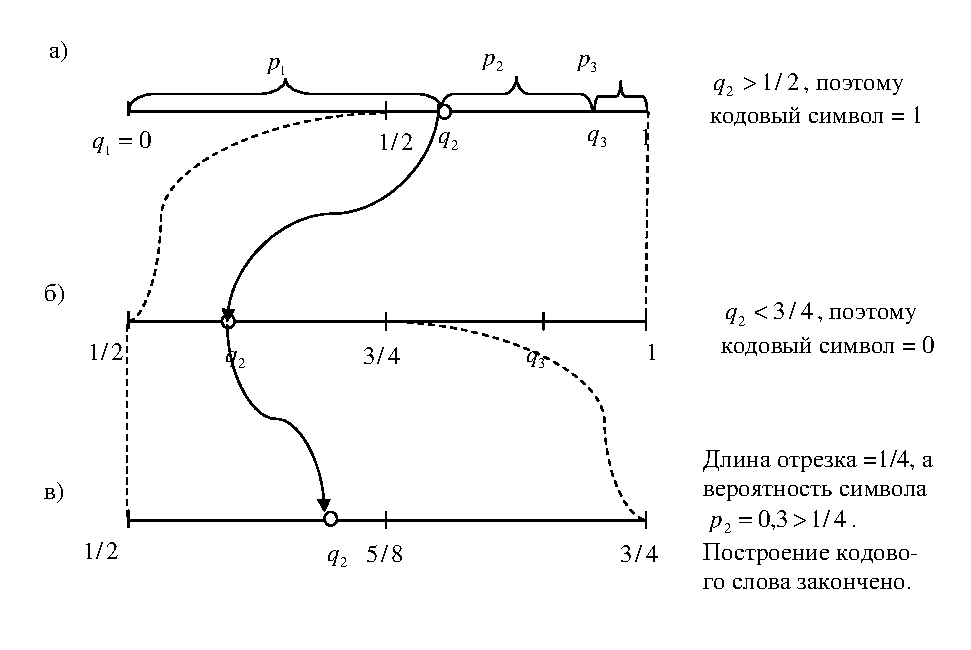
\includegraphics[width=1.0\textwidth]{fig2_7.eps}
\caption{Graphical interpretation of Shannon code }
\label{Shan_graph}
\end{minipage}
\end{figure}

\end{itemize}
\end{frame}

% ----------------------------Gilbert-Moore code-----------

\begin{frame}
\frametitle{Gilbert-Moore code}
\begin{itemize}    
% \footnotesize {
% \small{

    \begin{center}
    \begin{figure}
    \scalebox{0.75} {
    \begin{algorithm}[H]
    \dontprintsemicolon
      \KwIn{Alphabet size $M$, character probabilities $p_i, i=1,...,M$ }
      \KwOut{List of Gilbert-Moore code}
      \BlankLine
      \CommentSty{Auxiliary probabilities:}
      $q_{1}=0$;
      \For {$i=2$ \emph{\KwTo} $M$}
      {
      $q_i=q_{i-1}+p_{i-1}$;
      $\sigma_i=q_i+p_i/2$;
      }
      \BlankLine
      \CommentSty{Codewords:} 
      \For {$i=1$ \emph{\KwTo} $M$}
      {
      $\vec c_i\leftarrow $ первые
      $\left\lceil { - \log p_i } \right\rceil +1$ bits after comma in a binary number  $\sigma_i$.
      }
    \end{algorithm}
    }
    \caption{Gilbert-Moore code constriction algorithm}
    \label{alg_gm}
    \end{figure}
    \end{center}

\end{itemize}
\end{frame}


\begin{frame}
\frametitle{Gilbert-Moore code}
\begin{itemize}    
% \footnotesize {
% \small{

    \begin{table}[htbp]
    \caption{ Gilbert-Moore code eample} \label{tablGM}
    \begin{minipage}{\linewidth}
    \scalebox{0.75} {
    \begin{tabular}
     {|c|c|c|c|c|l|l|} \hline
     $x_m$ & $p_m$ & $q_m$ & $\sigma _m$ & $l_m$ & $\vec c_m$ \footnote
     {Gilbert-Moore codewords}
     &  $\tilde{\vec c}_m$ \footnote{Shannon codewords whithout character probability ordering}
     \\ \hline
     1& 0,1& 0,0=\small{[0,00000\dots ]}&
    0,05={\small{[0,00001\dots ]}}& 5& \small{00001}&\small 0000 \\
    \hline 2& 0,6& 0,1=\small[0,00011\dots ]& 0,40=\small[0,01100\dots
    ]& 2& \small 01&
    \small 0 \\
    \hline 3& 0,3& 0,7=\small[0,10110\ldots ]& 0,85=\small[0,11011\ldots
    ]& 3& \small 110&
    \small 10 \\
    \hline
    \end{tabular}
    }
    \end{minipage}
    \end{table}

\end{itemize}
\end{frame}


\begin{frame}
\frametitle{Gilbert-Moore code}
\begin{itemize}    
% \footnotesize {
\small{

    \item Consider
    \begin{eqnarray*}
    \sigma _j  + \frac{p_j }{2} - \sigma _i &=& \sum_{h = 1}^{j - 1}
    p_h - \sum_{h = 1}^{i - 1} p_h - \frac{p_i }{2}
    = \\
    &=& \sum_{h = i}^{j - 1} p_h  + \frac{p_j - p_i }{2} \ge
    \\
    &\ge& p_i + \frac{p_j - p_i }{2} =\\
     &=&\frac{p_j + p_i }{2} \ge
    \frac{\max \left\{ {p_i ,p_j } \right\}}{2}.
    \end{eqnarray*}

    \item For codeword length and its probability holds:
    \[
    l_m = \left\lceil { - \log \frac{p_m }{2}} \right\rceil \ge - \log \frac{p_m
    }{2}.
    \]
}
\end{itemize}
\end{frame}


\begin{frame}
\frametitle{Gilbert-Moore code}
\begin{itemize}    
% \footnotesize {
% \small{

    \item Thus,
    \[
    \sigma _j - \sigma _i \ge
    \frac{\max \{p_i ,p_j \}}{2} \ge 2^{ - \min \{l_i ,l_j \}},
    \]
    
    \item Average codeword length estimation
    \[
    \bar {l} < H + 2.
    \]

\end{itemize}
\end{frame}


\begin{frame}
\frametitle{Gilbert-Moore code}
\begin{itemize}    
% \footnotesize {
% \small{

\begin{figure}[ht]
\begin{minipage}{1.0\linewidth}
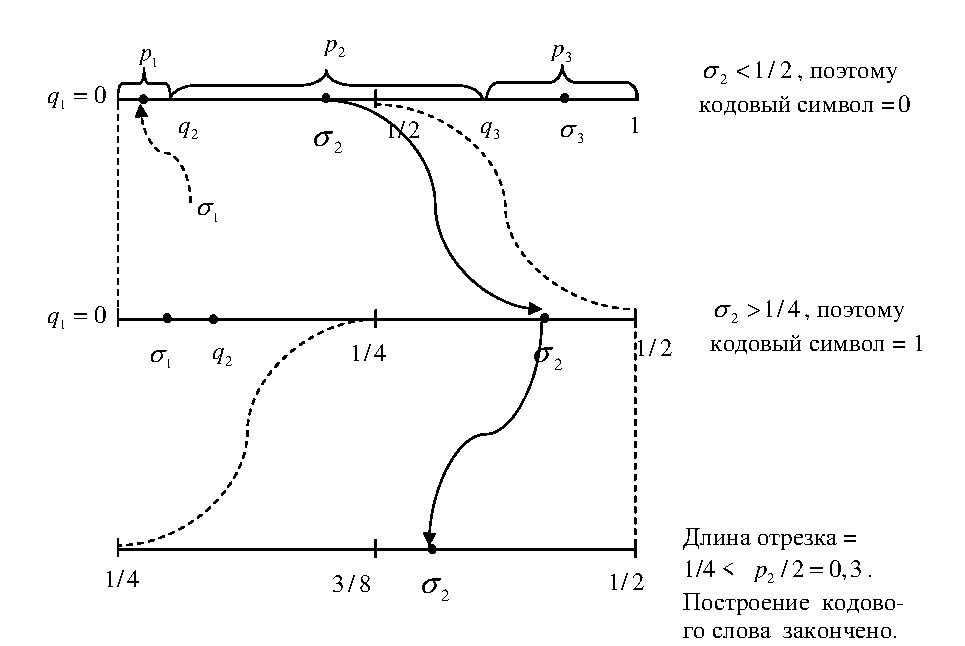
\includegraphics[width=1.0\textwidth]{fig2_8.eps}
\caption{Graphical interpretation of Gilbert-Moore code.}
\label{GM_graph}
\end{minipage}
\end{figure}

\end{itemize}
\end{frame}

% ----------------------Stationary source coding----------



\begin{frame}
\frametitle{Stationary source coding}
% \footnotesize {
\small{

    \begin{theorem} {Inverse Theorem} For DSS with entropy $H$ for any FV-coding holds:
    \[
    \bar {R} \ge H.
    \]
    \end{theorem}
    \textbf{Proof.}
    \begin{itemize}    
    \item consider $X^n$.
    \[
    {\rm {\bf M}}\left[ {l(\vec x)} \right] \ge H(X^n) = nH_n (X) \ge nH_\infty (X) = nH.
    \]
    \item $H_n (X)$ does not increase with increasing $n$. Thus, $\forall n$
    \[
    \bar {R}_n \ge H
    \]
    \item
    \[
    \bar {R} = \mathop {\inf }\limits_n R_n \ge H.
    \]
    \end{itemize}
}
\end{frame}


\begin{frame}
\frametitle{Stationary source coding}  
% \footnotesize {
\small{

    \begin{theorem}{Achievability theorem} For DSS with entropy $H$ and $\forall \delta > 0$ there exists FV-coding such that
    \[
    \bar {R} \le H + \delta .
    \]
    \end{theorem}
   
    \textbf{Proof. }
    \begin{equation}
    \label{p2eq8} {\rm {\bf M}}\left[ {l(\vec x)} \right] \le H(X^n) + 1
    = nH_n (X) + 1.
    \end{equation}
    
    \[
    \left| {H_n (X) - H} \right| \le \frac{\delta }{2},
    \]
    
    \begin{equation}
    \label{p2eq9} H_n (X) \le H + \frac{\delta }{2}, \quad n > n_1 .
    \end{equation}
}
\end{frame}

\begin{frame}
\frametitle{Stationary source coding}  
% \footnotesize {
\small{   
    \textbf{Proof. }
    \begin{equation}
    \label{p2eq10} \frac{1}{n} \le \frac{\delta }{2}.
    \end{equation}
    
    For $n \ge \max \{n_1 ,n_2 \}$, we get
    \begin{eqnarray*}
    \bar {R} &=& \mathop {\inf }\limits_m \bar {R}_m \le \\
    &\le& \bar {R}_n = \\
    &=& \frac{{\rm {\bf M}}\left[ {l(\vec x)} \right]}{n} \le \\
    &\le&  H_n (X) + \frac{1}{n} \le\\
    &\le& H + \frac{\delta }{2} + \frac{\delta }{2} =\\
    &=& H + \delta.
    \end{eqnarray*}
}
\end{frame}




\begin{frame}
\frametitle{Stationary source coding}
\begin{itemize}    
% \footnotesize {
% \small{

    \item For sequences $\vec x = (x_1 ,...,x_n )$, $\vec y = (y_1 ,...,y_n )$ denote $i$ to be the least index such that $x_i \ne y_i $.
    
    \item Then $\vec y \prec \vec x$, if $y_i \prec x_i$.
    
    \item Cumulative probability
    \begin{equation}
    \label{eq11} q(\vec x) = \sum\limits_{\vec y \prec \vec x}
    {p(\vec y} ),
    \end{equation}
    
    \item For memoryless source
    \[
    p(\vec x) = \prod\limits_{i = 1}^n {p(x_i )} .
    \]
    
    
\end{itemize}
\end{frame}


 \begin{frame}
\frametitle{Stationary source coding}
\begin{itemize}    
\footnotesize {
% \small{   

    \item For calculating $q(\vec x)$.
    \begin{eqnarray*}
     q(\vec x_1^n ) &=& \sum\limits_{\vec y_1^n \prec {\rm {\bf x}}_1^n }
    {p(\vec y_1^n )}=\\
    &=& \sum\limits_{\vec y_1^{n - 1} \prec \vec x_1^{n - 1} }
    {\sum\limits_{y_n } {p(\vec y_1^{n - 1} y_n )} } + \sum\limits_{\vec
    y_1^{n - 1} = {\rm {\bf x}}_1^{n - 1} } {\sum\limits_{y_n \prec x_n
    } {p(\vec y_1^{n - 1} y_n )}} = \\
    &=& \sum\limits_{\vec y_1^{n - 1} \prec \vec x_1^{n - 1} } {p(\vec
    y_1^{n - 1} )} + \sum\limits_{\vec y_1^{n - 1} =  \vec x_1^{n - 1} }
    {p(\vec y_1^{n - 1} )\sum\limits_{y_n \prec x_n } {p(y_n )} }= \\
    &=&q(\vec x_1^{n - 1} ) + p(\vec x_1^{n - 1} )q(x_n ) ,
    \end{eqnarray*}
    where $q(x_n )$ is cumulative probability of $x_n $.
    
    \item
    \begin{eqnarray}
    \label{eq12}
     q(\vec x_1^n ) &=& q(\vec x_1^{n - 1} ) + p(\vec x_1^{n
    - 1} )q(x_n ); \\
     p(\vec x_1^n ) &=& p(\vec x_1^{n - 1} )p(x_n ).
    \end{eqnarray}
}
\end{itemize}
\end{frame}

\begin{frame}
\frametitle{Stationary source coding}   
% \footnotesize {
% \small{

    \begin{center}
    \begin{figure}
    \scalebox{0.75} {
    \begin{algorithm}[H]
    \dontprintsemicolon
      \KwIn
      {
       Alphabet size $M$
       character probabilities $p_i, i=1,...,M$
       length  $n$
       sequence at output $(x_1,...,x_n)$,
       }
      \KwOut{Arithmetic codeword}
      \BlankLine
      \CommentSty{Cumulative probabilities:}
      $q_{1}=0$;
      \For {$i=2$ \emph{\KwTo} $M$}
      {
      $q_i=q_{i-1}+p_{i-1}$;
      }
      \BlankLine
      \CommentSty{Coding:}
      \For {$i=1$ \emph{\KwTo} $n$}
      {
      $ F \leftarrow F + q(x_i )G $;
      $ G \leftarrow p(x_i )G $;.
      }
      \BlankLine
      \CommentSty{Codeword creation:}
      $\vec c\leftarrow $ first
      $\left\lceil { - \log G } \right\rceil +1$ bits after comma in a binary number $F+G/2$.
    \end{algorithm}
    }
    \caption{Arithmetic coding algorithm}
    \label{alg_arcod}
    \end{figure}
    \end{center}
\end{frame}


\begin{frame}
\frametitle{Stationary source coding}   
% \footnotesize {
% \small{

    \begin{table}[htbp]
    \caption{Arithmetic coding of sequence}
    \label{tablAC}
    \begin{minipage}{\linewidth}
    \begin{center}
    \scalebox{0.75}{
    \begin{tabular}{|c|c|c|c|c|c|}
    \hline Шаг $i$& $x_i $& $p(x_i )$& $q(x_i )$& $F$&$G$ \\     \hline
    0& -& -& -& 0,0000& 1,0000 \\\hline 1& $b$& 0,6& 0,1& 0,1000&
    0,6000 \\
    2& $c$& 0,3& 0,7& 0,5200&
    0,1800 \\
    \hline 3& $b$& 0,6& 0,1& 0,5380&
    0,1080 \\
    \hline 4& $a$& 0,1& 0,0& 0,5380&
    0,0108 \\
    \hline 5& $b$& 0,6& 0,1& 0,5391&
    0,0065 \\
    \hline \raisebox{-1.50ex}[0cm][0cm]{6}& \multicolumn{5}{l|}{Codeword length $\left\lceil -
    \log G + 1 \right\rceil = 9$}\\ %\cline{2-6}
    &\multicolumn{5}{l|}
    {Codeword $F + G / 2 = 0,5423...\to$ }\\ &\multicolumn{5}{l|} {
    $\to \hat {F} = 0,541 \to 100010101$}
    \\
    \hline
    \end{tabular}
    }
    \end{center}
    \end{minipage}
    \end{table}
\end{frame}


\begin{frame}
\frametitle{Stationary source coding}
\begin{itemize}    
% \footnotesize {
% \small{

\begin{figure}[htbp]
\begin{minipage}{0.9\linewidth}
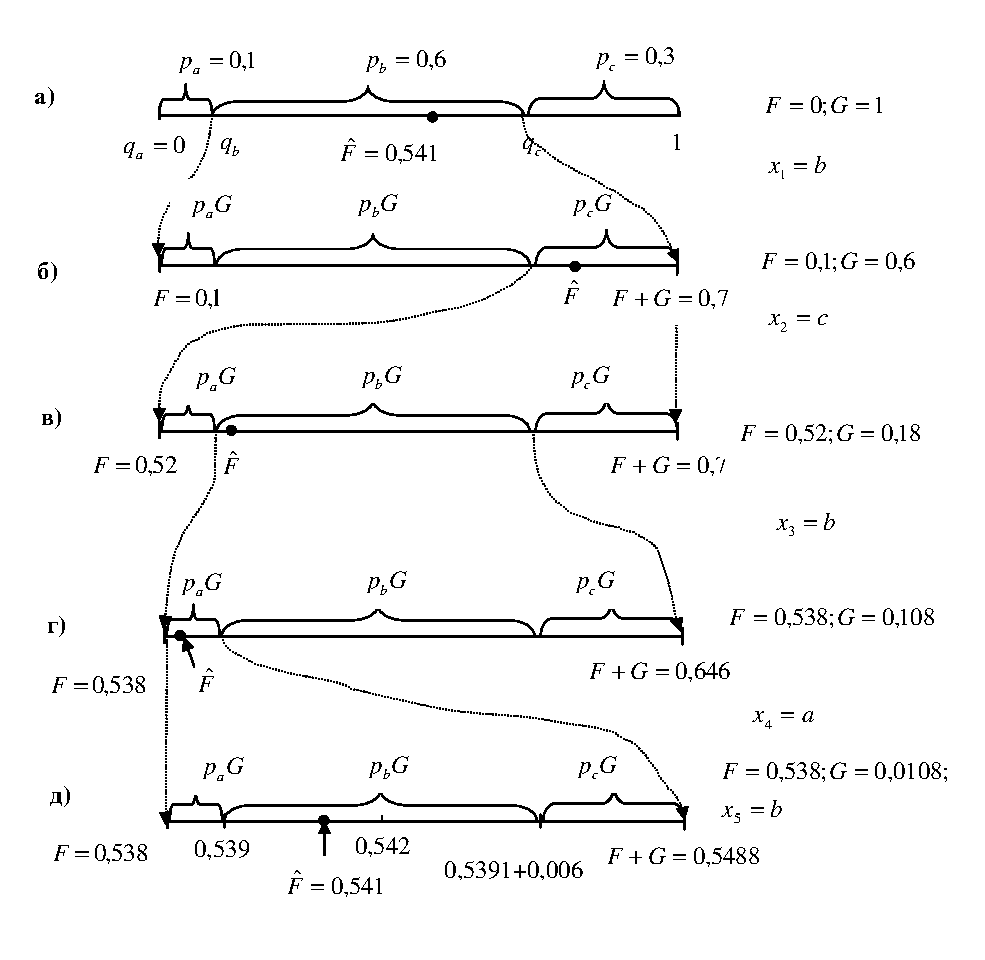
\includegraphics[width=1.0\textwidth]{fig2_9.eps}
\caption{Graphical interpretation of arithmetic coding }
\label{AC_graph}
\end{minipage}
\end{figure}


\end{itemize}
\end{frame}



\begin{frame}
\frametitle{Stationary source coding}   
% \footnotesize {
% \small{

    \begin{center}
    \begin{figure}
    \begin{algorithm}[H]
    \dontprintsemicolon
      \KwIn
      {
       Alphabet size $M$
       cumulative probabilities $q_i, i=1,...,M$\;
       decode input $\hat {\sigma }$.
       }
      \KwOut{Decoded character $x$}
      \BlankLine
      \CommentSty{Init:}
      $q_{M+1}=1$;
      $m = 1$.\;
      \BlankLine
      \CommentSty{character search:} 
      \While {$q_{m + 1} < \hat {\sigma }$}
      {
        $m \leftarrow m + 1$.
      }
      \BlankLine
      \CommentSty{Result:} 
      $x=x_m$
      \end{algorithm}
    \caption{Gilbert-Moore decoding algorithm}
    \label{Alg_dec_GM}
    \end{figure}
    \end{center}
\end{frame}



\begin{frame}
\frametitle{Stationary source coding}   
% \footnotesize {
% \small{

    \begin{center}
    \begin{figure}
    \scalebox{0.65}{
    \begin{algorithm}[H]
    \dontprintsemicolon
      \KwIn
      {
       Alphabet size $M$\;
       character probabilities $\{p_1 ,...,p_M \}$\,cumulative probabilities $q_i, i=1,...,M$
       decoded sequence length $n$, codeword as a number $\hat F$.
      }
      \KwOut{Decoded character sequence $(x_1,...,x_n)$}
      \BlankLine
      \CommentSty{Init:}  $q_{M+1}=1$;  $S = 0$;  $G = 1$.\;
      \BlankLine
      \CommentSty{Decoding:} \;
      \For {$i=1$ \emph{\KwTo} $n$}
      {
        $j=1$;
    
        \While {$S + q_{j + 1} G < \hat F$ }
        {
             $j \leftarrow j + 1$.
        }
        $ S \leftarrow S + q_j G $;\;
        $ G \leftarrow p_j G $;\;
        $ x_i = j $.\;
      }
      \BlankLine
      \CommentSty{Result: sequence} $(x_1,...,x_n)$;
      \end{algorithm}
      }
    \caption{Arithmetic code decoding algorithm}
    \label{Alg_ar_dec}

    \end{figure}
    \end{center}

\end{frame}



\begin{frame}
\frametitle{Stationary source coding}   
% \footnotesize {
\small{

    \begin{table}[htbp]
    \caption{$X = \{a,b,c\}$. $p_a = 0,1$, $p_b = 0,6$, $p_c = 0,3$. $0100010101$}
    \begin{minipage}{\linewidth}
    \begin{center}
    \scalebox{0.65}{
    \begin{tabular}
    {|c|c|c|c|c|c|c|c|} \hline \raisebox{-1.00ex}{\small Step}&
    \raisebox{-1.00ex}{$S$}& \raisebox{-1.00ex}{$G$} &{\tiny Hypotesis}&
    \raisebox{-1.00ex}{$q(x)$}& \raisebox{-1.00ex}{$S + qG$}& \tiny
    Decision& \raisebox{-1.00ex}{$p(x)$} \\
           & & & $x$& & & $x_i $& \\\hline
    0&\multicolumn{7}{c|}{100010101$ \to \hat {F} = $0,541}  \\
    \hline \raisebox{-3.00ex}[0cm][0cm]{1}&
    \raisebox{-3.00ex}[0cm][0cm]{0,0000}&
    \raisebox{-3.00ex}[0cm][0cm]{1,0000}& $a$& 0,0& 0,0000$ < \hat {F}$&
    \raisebox{-3.00ex}[0cm][0cm]{$b$}&
    \raisebox{-3.00ex}[0cm][0cm]{0,6} \\
    \cline{4-6}
     & & &$b$&0,1&\textbf{0,1000}$ < \hat {F}$& &  \\ \cline{4-6}
     & & &$c$&0,7&0,7000$ > \hat {F}$& &  \\ \hline
    \raisebox{-3.00ex}[0cm][0cm]{2}&
    \raisebox{-3.00ex}[0cm][0cm]{0,1000}&
    \raisebox{-3.00ex}[0cm][0cm]{0,6000}& $a$& 0,0& 0,1000$ < \hat {F}$&
    \raisebox{-3.00ex}[0cm][0cm]{$c$}& \raisebox{-3.00ex}[0cm][0cm]{0,3}
    \\ \cline{4-6}
     & & & $b$& 0,1& 0,1600$ < \hat {F}$&  &   \\ \cline{4-6}
     & & & $c$& 0,7& \textbf{0,5200}$ < \hat {F}$&  &   \\ \hline
    \raisebox{-3.00ex}[0cm][0cm]{3}&
    \raisebox{-3.00ex}[0cm][0cm]{0,5200}&
    \raisebox{-3.00ex}[0cm][0cm]{0,1800}& $a$& 0,0& 0,5200$ < \hat {F}$&
    \raisebox{-3.00ex}[0cm][0cm]{$b$}& \raisebox{-3.00ex}[0cm][0cm]{0,6}
    \\ \cline{4-6}
     & & &$b$&0,1&\textbf{0,5380}$ < \hat {F}$& &  \\\cline{4-6}
     & & &$c$&0,7&0,6460$ > \hat {F}$& &  \\\hline
    \raisebox{-1.50ex}[0cm][0cm]{4}&
    \raisebox{-1.50ex}[0cm][0cm]{0,5380}&
    \raisebox{-1.50ex}[0cm][0cm]{0,1080}& $a$& 0,0& \textbf{0,5380}$ <
    \hat {F}$& \raisebox{-1.50ex}[0cm][0cm]{$a$}&
    \raisebox{-1.50ex}[0cm][0cm]{0,1} \\ \cline{4-6}
     & & &$b$&0,1&0,5488$ > \hat {F}$& &  \\\hline
    \raisebox{-3.00ex}[0cm][0cm]{5}&
    \raisebox{-3.00ex}[0cm][0cm]{0,5380}&
    \raisebox{-3.00ex}[0cm][0cm]{0,0108}& $a$& 0,0& 0,5380$ < \hat {F}$&
    \raisebox{-3.00ex}[0cm][0cm]{$b$}&
    \raisebox{-3.00ex}[0cm][0cm]{0,6} \\
    \cline{4-6}
     & & & $b$& 0,1& \textbf{0,5391}$ < \hat {F}$&  &   \\ \cline{4-6}
     & & & $c$& 0,7& 0,5456$ > \hat {F}$&  &   \\  \hline
    \end{tabular}
    }
    \end{center}
    \end{minipage}
    \label{tabARD}
    \end{table}
}
\end{frame}


\begin{frame}
\frametitle{Stationary source coding}    
% \footnotesize {
% \small{
  \begin{multicols}{2}
  \includegraphics[width=0.28\textwidth]{fig_ar_encoder.eps}
  
  \columnbreak
  
  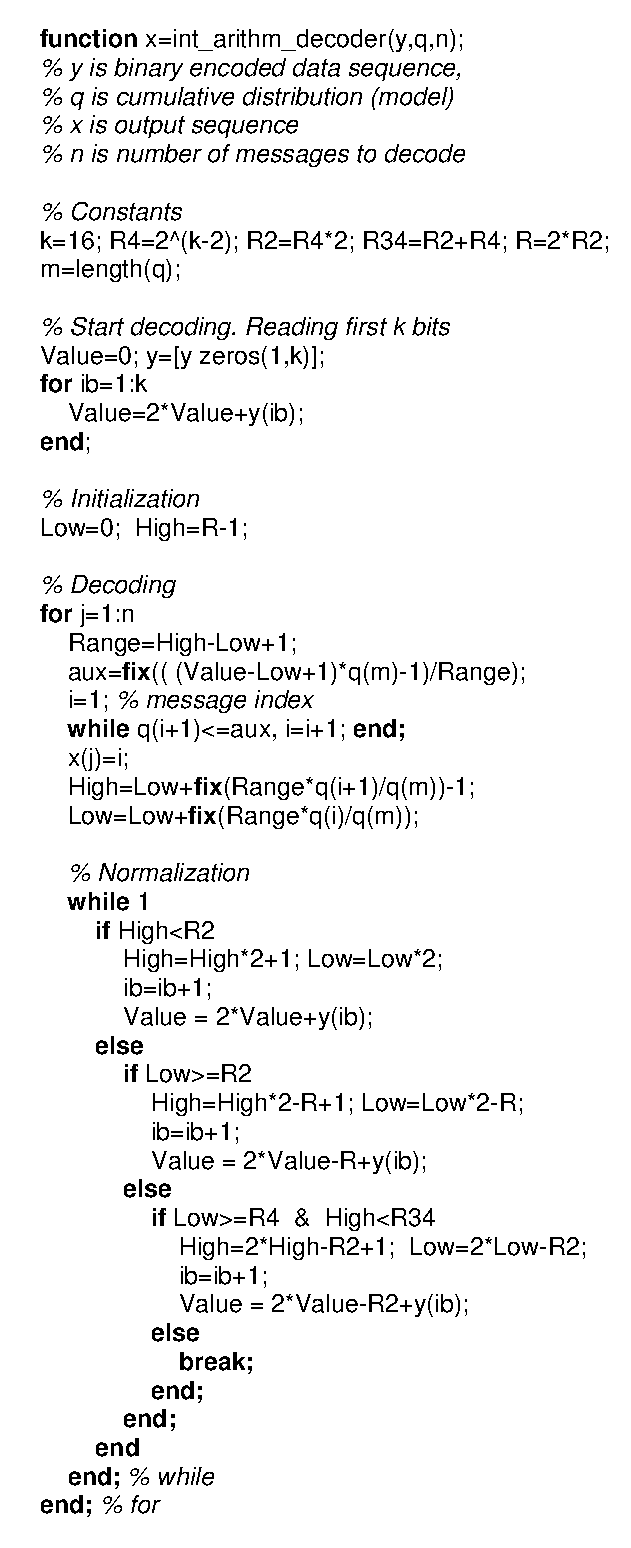
\includegraphics[width=0.28\textwidth]{fig_ar_decoder.eps}
  
  \end{multicols}
\end{frame}

\end{document} 